\chapter{Inner Product Spaces}

\section{Inner product spaces}


\dfn{Inner Products}{

	Let \(V\) be a vector space over \(\FF\), with \(\FF = \RR\) or \(\FF = \CC\).

	The inner product:

	\begin{align*}
		\left<\,,\,\right> : V \times V & \to \FF                     \\
		(v, w)                          & \mapsto \left< v, w \right>
	\end{align*}

	Such that:

	\begin{enumerate}[wide]
		\item \(\left< v, v \right> \in \RR\) and \(\left< v, v \right> \ge 0\) for all \(v \in V\)
		\item \(\left< v, v \right> = 0 \iff v = \vec{0}_{v}\)
		\item \(\left< u + w, v \right> = \left< u, v \right> + \left< w, v \right>\) for all \(u, w, v \in V\)
		\item \(\left< \lambda \cdot_{v} v, w \right> = \lambda \cdot_{\FF} \left< v, w \right>\) for all \(\lambda \in \FF\) and \(v, w \in V\)
		\item \(\left< u, v \right> = \overline{\left< v, u \right>}\) for all \(u, v \in V\)
	\end{enumerate}
}

\ex{}{
	\begin{enumerate}[label=(\roman*)]
		\item Let \(V = \RR^{n}\) with \(\FF = \RR\) and \(\left<\,,\, \right> = \) the dot product.

		      Then,

		      \[
			      \left< (x_{1}, \ldots, x_{n}), (y_{1}, \ldots, y_{n}) \right> \coloneq x_{1}y_{1} + \ldots + x_{n}y_{n}
		      \]

		      And:

		      \[
			      \left< (x_{1}, \ldots, x_{n}), (x_{1}, \ldots, x_{n}) \right> = x_{1}^{2} + \ldots + x_{n}^{2} = 0 \iff (x_{1}, \ldots, x_{n}) = (0, \ldots, 0)
		      \]

		\item Let \(V = \CC^{n}\) with \(\FF = \CC\) and \(\left<\,,\, \right> = \) the dot product.

		      Then,

		      \[
			      \left< (z_{1}, \ldots, z_{n}), (w_{1}, \ldots, w_{n}) \right> \coloneq z_{1}\overline{w_{1}} + \ldots + z_{n}\overline{w_{n}}
		      \]

		      And:

		      \[
			      \left< (z_{1}, \ldots, z_{n}), (z_{1}, \ldots, z_{n}) \right> = z_1\overline{z_1} + \ldots + z_n\overline{z_n} = \left\lvert z_1 \right\rvert^{2} + \ldots + \left\lvert z_n \right\rvert^{2} \ge 0
		      \]
		\item \(V = P(\RR)\) with \(\FF = \RR\) and \(\left<\,,\, \right> = \) the integral.

		      Then,

		      \[
			      \left< p, q \right> \coloneq \int_{0}^{\infty} p(x)q(x) \cdot e_{-x} dx
		      \]
		\item \(V = \left\{ f: [-1, 1] \to \RR \mid f \text{ is continuous} \right\}\) with \(\FF = \RR\) and \(\left<\,,\, \right> = \) the integral.

		      Then,

		      \[
			      \left< f, g \right> \coloneq \int_{-1}^{1} f(x)g(x) dx
		      \]

	\end{enumerate}
}

\dfn{Inner product space}{
	Vector space with an inner product is called an inner product space.

	Consequences of axoims:

	\begin{enumerate}[label=(\roman*)]
		\item Fix \(u \in V\). Define:


		      \begin{align*}
			      T_{u} : V & \to \FF                     \\
			      v         & \mapsto \left< v, u \right>
		      \end{align*}

		      Then \(T_{u}\) is a linear map.

		      Additivity:

		      \[
			      T_{u}(v + w) = \left< v + w, u \right> = \left< v, u \right> + \left< w, u \right> = T_{u}(v) + T_{u}(w)
		      \]

		      Homogeneity:

		      \[
			      T_{u}(\lambda \cdot_{v} v) = \left< \lambda \cdot_{v} v, u \right> = \lambda \cdot_{\FF} \left< v, u \right> = \lambda \cdot_{\FF} T_{u}(v)
		      \]

		\item \(\left< \vec{0}_{v}, v\right> = 0_{\FF} : \left< \vec{0}_{v} , v \right> = T_{v}(\vec{0}_{v}) = 0_{\FF}\)
		\item \(\left( \left< v, u + w \right> = \left< v, u \right> + \left< v, w \right> \right)\):

		      Reasoning:

		      \begin{align*}
			      \left< v, u + w \right> & = \overline{\left< u + w, v \right>}                                                    \\
			                              & = \overline{\left< u, v \right> + \left< w, v \right>}                                  \\
			                              & = \overline{\left< u, v \right>} + \overline{\left< w, v \right>}                       \\
			                              & = \overline{\overline{\left< v, u \right>}} + \overline{\overline{\left< v, w \right>}} \\
			                              & = \left< v, u \right> + \left< v, w \right>
		      \end{align*}

		\item \(\left< v, \vec{0}_{v} \right> = 0_{\FF} : \left< v, \vec{0}_{v} \right> = \overline{\left< \vec{0}_{v}, v \right>} = \overline{0_{\FF}} = 0_{\FF}\)
		\item \(\left<v, \lambda \cdot w \right> = \overline{\lambda} \cdot \left< v, w \right>\):

		      Reason:
		      \begin{align*}
			      \left< v, \lambda \cdot w \right> & = \overline{\left< \lambda \cdot w, v \right>}            \\
			                                        & = \overline{\lambda \cdot \left< w, v \right>}            \\
			                                        & = \overline{\lambda} \cdot \overline{\left< w, v \right>} \\
			                                        & = \overline{\lambda} \cdot \left< v, w \right>
		      \end{align*}
	\end{enumerate}
}

\dfn{}{
	Inner products is approx ``size of a vector''.

	Norm:

	\[
		\left\lvert v \right\rvert \coloneq \sqrt{\left< v, v \right>}
	\]
}

\ex{}{
	\begin{enumerate}[wide]
		\item \(V = \RR^{n}, \FF=\RR, \left<\,,\, \right> = \) dot product.

		      \[
			      \left\lVert (x_{1}, \ldots, x_{n}) \right\rVert = \sqrt{x_{1}^{2} + \ldots + x_{n}^{2}}
		      \]
		\item \(V = \left\{ f: [-1, 1] \to \RR \mid f \text{ is continuous} \right\}, \FF=\RR, \left< f(x), g(x) \right> = \int_{-1}^{1} f(x)g(x) dx\)

		      \[
			      \left\lVert f \right\rVert = \sqrt{\int_{-1}^{1} f(x)^{2} dx}
		      \]


		      Meaning \( \left\lVert f - g_{n} \right\rVert \to 0 \) as \(n \to \infty\).
	\end{enumerate}
}

\mclm{For norms}{

	\begin{align*}
		\left\lVert v \right\rVert = 0_{\FF} & \iff \sqrt{ \left<v, v \right> } = 0_{\FF} \\
		                                     & \iff \left<v, v \right> = 0_{\FF}          \\
		                                     & \iff v = \vec{0}_{v}
	\end{align*}
}

\dfn{orthogonal}{
	Two vectors \(u, v\) are orthogonal if \(\left< u, v \right> = 0_{\FF}\).
}

\ex{}{
	Let \(V = \RR^{2}\):

	\begin{align*}
		\left< (x_1, y_1), (x_2, y_2) \right>  = 0 & \iff x_1x_2 + y_1y_2 = 0                                          \\
		                                           & \iff \frac{x_2}{y_2} = -\frac{y_1}{x_1}                           \\
		                                           & \iff (x_1, y_1) \text{ and } (x_2, y_2) \text{ are perpendicular}
	\end{align*}
}

\thm{Pythagoras}{
	Suppose \(u, v \in V\) are orthogonal. Then:


	\[
		\left\lVert u + v \right\rVert^{2} = \left\lVert u \right\rVert^{2} + \left\lVert v \right\rVert^{2}
	\]

	\pf{Proof}{
		\begin{align*}
			\left\lVert u + v \right\rVert^{2} & = \left< u + v, u + v \right>                                                           \\
			                                   & = \left< u, u + v \right> + \left< v, u + v \right>                                     \\
			                                   & = \left< u, u \right> + \left< u, v \right> + \left< v, u \right> + \left< v, v \right> \\
			                                   & = \left< u, u \right> + 0_{\FF} + 0_{\FF} + \left< v, v \right>                         \\
			                                   & = \left\lVert u \right\rVert^{2} + \left\lVert v \right\rVert^{2}
		\end{align*}
	}
}

\mclm{Loose End}{
	\[
		\left\lVert \lambda v \right\rVert = \left\lvert \lambda \right\rvert \cdot \left\lVert v \right\rVert
	\]

	As both are non-negative.

	\pf{Proof}{
		\begin{align*}
			\left\lVert \lambda v \right\rVert & = \sqrt{\left< \lambda v, \lambda v \right>}                            \\
			                                   & = \sqrt{\lambda \cdot \overline{\lambda} \cdot \left< v, v \right>}     \\
			                                   & = \sqrt{\left\lvert \lambda \right\rvert^{2} \cdot \left< v, v \right>} \\
			                                   & = \left\lvert \lambda \right\rvert \cdot \sqrt{\left< v, v \right>}     \\
			                                   & = \left\lvert \lambda \right\rvert \cdot \left\lVert v \right\rVert
		\end{align*}
	}
}

\mclm{Orthonormal Decompositions}{

	Given:

	\begin{tikzpicture}
		\draw[->] (0, 0) -- (2, 1) node[anchor=south] {$u$};
		\draw[->] (0, 0) -- (1, 0) node[anchor=west] {$v$};
	\end{tikzpicture}

	Find \(c \in \FF, w \in V\) such that we complete the triangle, i.e. \(u = c \cdot v + w\).

	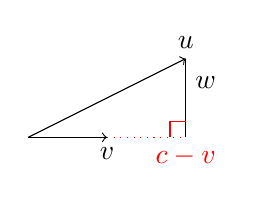
\begin{tikzpicture}
		\draw[->] (0, 0) -- (2, 1) node[anchor=south] {$u$};
		\draw[->] (0, 0) -- (1, 0) node[anchor=north] {$v$};
		\draw (2, 0) -- (2, 1) node[midway, anchor=south west] {$w$};
		\draw[dotted, red] (1, 0) -- (2, 0) node[anchor=north] {$c - v$};
		\draw[red] (1.8, 0) -- (1.8, 0.2) -- (2, 0.2);
	\end{tikzpicture}

	Want:

	\begin{align*}
		\left<w, v \right> & \iff \left<u - c \cdot v, v \right> = 0                                 \\
		                   & \iff \left<u, v \right> - c \cdot \left<v, v \right> = 0                \\
		                   & \iff \left< u, v \right> - c \cdot \left\lVert v \right\rVert^{2} = 0   \\
		                   & \implies c = \frac{\left< u, v \right>}{\left\lVert v \right\rVert^{2}} \\
	\end{align*}

	\nt{

		\[
			w = u - cv = u - \frac{\left< u, v \right>}{\left\lVert v \right\rVert^{2}} \cdot v
		\]

		Where \(v\) and \(w\) are orthogonal.
	}
}

\thm{Cauchy-Schwarz inequality}{
	Suppose that \(V\) is an inner product space and \(u, v \in V\). Then:

	\[
		\left\lvert \left< u, v \right> \right\rvert \le \left\lVert u \right\rVert \cdot \left\lVert v \right\rVert
	\]

	With equality if and only if \(u\) and \(v\) are linearly dependent.

	\pf{Proof}{
		If \(v = \vec{0_{v}} \), then both sides are \(0_{\FF}\).

		\nt{
			In this case equality holds and \(u, v\) are linearly dependent.
		}

		If \(v \neq \vec{0_{v}} \), then \(v\) and \(w \coloneq u - \frac{\left< u, v \right>}{\left\lVert v \right\rVert^{2}} \cdot v\) are orthogonal.

		Which means so are \(\alpha \cdot v\) and \(w\) for any \(\alpha \in \FF\).

		Recall that Pythagoras:

		\[
			\left\lVert w + \alpha \cdot v \right\rVert^{2} = \left\lVert w \right\rVert^{2} + \left\lVert \alpha v \right\rVert^{2} = \left\lVert w \right\rVert^{2} + \left\lvert \alpha \right\rvert^{2} \cdot \left\lVert v \right\rVert^{2}
		\]



		Pick \(\alpha = \frac{\left< u, v \right>}{\left\lVert v \right\rVert^{2}}\), so that \(w + \alpha v = u\)


		This implies that:

		\[
			\left\lVert u \right\rVert^{2} = \left\lVert w \right\rVert^{2} + \left\lvert \frac{\left< u, v \right>}{\left\lVert v \right\rVert^{2}} \right\rvert^{2} \cdot \left\lVert v \right\rVert^{2}
		\]

		Where the right term of the sum is:

		\[
			\frac{\left\lvert \left<u, v \right> \right\rvert^{2}}{\left\lVert v \right\rVert^{4}} \cdot \left\lVert v \right\rVert^{2}
		\]

		Which is:

		\[
			\left\lVert v \right\rVert^{2} = \left\lVert w \right\rVert^{2} + \frac{\left\lvert \left<u, v \right> \right\rvert^{2}}{\left\lVert v \right\rVert^{2}} \geq \frac{\left\lvert \left<u, v \right> \right\rvert^{2}}{\left\lVert v \right\rVert^{2}}
		\]

		So we get:

		\[
			\left\lVert v \right\rVert^{2} \geq \frac{\left\lvert \left<u, v \right> \right\rvert^{2}}{\left\lVert v \right\rVert^{2}} \implies \left\lVert u \right\rVert \cdot \left\lVert v \right\rVert \geq \left\lvert \left<u, v \right> \right\rvert
		\]

		Notice that equality holds if and only if:

		\begin{align*}
			\left\lVert w \right\rVert = 0 & \iff w = \vec{0_{v}}                                                                                                 \\
			                               & \iff u = \frac{\left< u, v \right>}{\left\lVert v \right\rVert^{2}} \cdot v = 0                                      \\
			                               & \iff u = \frac{\left< u, v \right>}{\left\lVert v \right\rVert^{2}} \cdot v \iff u, v \text{ are linearly dependent}
		\end{align*}



	}
}

\ex{}{
	\begin{enumerate}[wide]
		\item Let \(V = \RR^{n}, \FF = \RR, \left<\,,\, \right> = \) dot product.

		      \begin{align*}
			      \vec{x}  = (x_1, \ldots, x_{n}) \\
			      \vec{y}  = (y_1, \ldots, y_{n}) \\
		      \end{align*}

		      C.S. tell us:

		      \begin{align*}
			      \left\lvert \left< \vec{x}, \vec{y} \right> \right\rvert^{2} & \leq \left\lVert \vec{x} \right\rVert^{2} \cdot \left\lVert \vec{y} \right\rVert^{2} \\
			      (x_1y_1 + \ldots + x_{n}y_{n})^{2}                           & \leq (x_{1}^{2} + \ldots + x_{n}^{2}) \cdot (y_{1}^{2} + \ldots + y_{n}^{2})         \\
		      \end{align*}
		\item Let \(V = \left\{ f : [-1, 1] \to \RR \mid f \text{ is continuous} \right\}, \FF = \RR, \left< f, g \right> = \int_{-1}^{1} f(x)g(x) dx\).

		      By C.S., we know that:

		      \[
			      \left\lvert \left< f, g \right> \right\rvert^{2} \leq \left\lVert f \right\rVert^{2} \cdot \left\lVert g \right\rVert^{2}
		      \]

		      Thus:

		      \begin{align*}
			      \left(\int_{-1}^{1} f(x)g(x) dx\right)^{2} & \leq \left(\int_{-1}^{1} f(x)^{2} dx\right) \cdot \left(\int_{-1}^{1} g(x)^{2} dx\right) \\
		      \end{align*}
	\end{enumerate}
}

\thm{Triangle Inequality}{

	Given \(u, v\) in an inner product space \(V\), we have:

	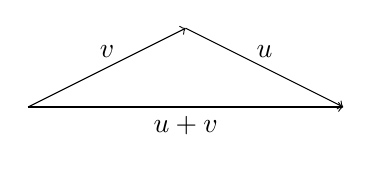
\begin{tikzpicture}
		\draw[->] (0, 0) -- (2, 1) node[midway, above] {$v$};
		\draw[->] (2, 1) -- (4, 0) node[midway, above] {$u$};
		\draw[->] (0, 0) -- (4, 0) node[midway, below] {$u + v$};
	\end{tikzpicture}

	The triangle inequality states that:

	\[
		\left\lVert u + v \right\rVert \leq \left\lVert u \right\rVert + \left\lVert v \right\rVert
	\]

	\pf{Proof}{

		\begin{align*}
			\left\lVert u + v \right\rVert^{2} & = \left< u + v, u + v \right>                                                                                                                         \\
			                                   & = \left< u, u\right> + \left< u, v \right> + \left< v, u \right> + \left< v, v \right>                                                                \\
			                                   & = \left\lVert u \right\rVert^{2} + \left<u, v \right>+ \overline{\left<u, v \right>} + \left\lVert v \right\rVert^{2}                                 \\
			                                   & = \left\lVert u \right\rVert^{2} + 2 \cdot \operatorname{Re}\left<u, v \right> + \left\lVert v \right\rVert^{2} \text{ as } (a + bi) + (a - bi) = 2a  \\
			&\le \left\lVert u \right\rVert^{2} + 2 \cdot \left\lvert \left< u, v \right> \right\rvert + \left\lVert v \right\rVert^{2}\text{ by } \star               \\
			&\le \left\lVert u \right\rVert^{2} + 2 \cdot \left\lVert u \right\rVert \cdot \left\lVert v \right\rVert + \left\lVert v \right\rVert^{2} \text{ by C.S.} \\
			&= \left(\left\lVert u \right\rVert + \left\lVert v \right\rVert\right)^{2}
		\end{align*}

		Thus, we get:

		\begin{align*}
			\left\lVert u + v \right\rVert^{2} & \leq \left(\left\lVert u \right\rVert + \left\lVert v \right\rVert\right)^{2} \\
			\left\lVert u + v \right\rVert     & \leq \left\lVert u \right\rVert + \left\lVert v \right\rVert
		\end{align*}

		So why is \(\star\) true?

		\begin{align*}
			\left< u, v \right> = a + bi &\implies \left\lvert \left< u, v \right> \right\rvert = \sqrt{a^{2} + b^{2}} \\
			\operatorname{Re}\left<u, v \right> &= a
		\end{align*}

		But why is \(a \leq \sqrt{a^{2} + b^{2}}\)?

		True since:

		\begin{align*}
			a &\le \left\lvert a \right\rvert \\
			  &= \sqrt{a^{2}} \\
			  &\le \sqrt{a^{2} + b^{2}}
		\end{align*}

		Which means the triangle inequality holds.
	}
}

\ex{}{
	Let \(V = \RR^{n}, \vec{x} = (x_1, \ldots, x_{n}), \vec{y} = (y_1, \ldots, y_{n})\).

	We have:

	\[
		\left\lVert \vec{x} + \vec{y} \right\rVert^{2} = \left\lVert \vec{x} \right\rVert^{2} + 2 \cdot \left< \vec{x}, \vec{y} \right> + \left\lVert \vec{y} \right\rVert^{2}
	\] 

	Thus:

	\begin{align*}
		\sum_{i=1}^{n} (x_{i} + y_{i})^{2} &\leq \left(\sqrt{\sum_{i=1}^{n} x_{i}^{2}} + \sqrt{\sum_{i=1}^{n} y_{i}^{2}}\right)^{2} \\
		&= \sum_{i=1}^{n} x_{i}^{2} + 2 \cdot \sqrt{\sum_{i=1}^{n} x_{i}^{2}} \cdot \sqrt{\sum_{i=1}^{n} y_{i}^{2}} + \sum_{i=1}^{n} y_{i}^{2} \\
	\end{align*}
}


\section{Orthonormal bases}

\dfn{}{
	Let \(V\) be an inner product space over \(\FF\).

	Let \(e_1, \ldots, e_{n} \) be a list of vectors in \(V\).

	Then we say \(\left\{ e_1, \ldots, e_{n} \right\}\) is an orthogonal list if:

	\[
		\left< e_i, e_j \right> = \delta_{ij} \coloneq \begin{cases}
			1_{\FF} & i = j    \\
			0_{\FF} & i \neq j
		\end{cases}
	\] 

	E.g.

	\begin{align*}
		\left( \frac{1}{\sqrt{3} }, \frac{1}{\sqrt{3} }, \frac{1}{\sqrt{3} } \right), \left( -\frac{1}{\sqrt{2} }, \frac{1}{\sqrt{2} }, 0 \right) \in \RR^{3} \\
	\end{align*}

	We normalize the vectors to get a length of \(1\).

	If an orthogonal list is also a basis, then the following holds:

	\begin{align*}
		\left\lVert a_1 e_1 + \ldots + a_{n} e_{n} \right\rVert^{2} &= \left< a_1 e_1 + \ldots + a_{n} e_{n}, a_1 e_1 + \ldots + a_{n} e_{n} \right> \\
		&= \left<a_1 e_1, a_1 e_1\right> + \ldots + \left<a_{n} e_{n}, a_{n} e_{n}\right> \\
		&= a_1 \cdot \overline{a_1} \left<e_1, e_1 \right> + \ldots + a_{n} \cdot \overline{a_{n}} \left<e_{n}, e_{n}\right> \\
		&= \left\lvert a_1 \right\rvert^{2} + \ldots + \left\lvert a_{n} \right\rvert^{2} \\
	\end{align*}

	A list of orgthogonal vectors is linearly independent, but might not span.
}




\dfn{}{

	\(V\) is an inner product space over \(\RR\) or \(\CC\).

	Then we say \(\left\{ V_1, \ldots, V_{n} \right\}\) is an orthonormal if :

	\[
		\left< V_{i}, V_{j} \right> = \begin{cases}
			1_{\FF} & i = j    \\
			0_{\FF} & i \neq j
		\end{cases}
	\]

}

\clm{}{}{
Suppose \(\left\{ V_{1}, \ldots, V_{n} \right\}\) is orthonormal, then \(\left\{ V_{1}, \ldots, V_{n} \right\}\) is linearly independent.

\pf{Proof}{
	Suppose there are some scalars \(c_1, \ldots, c_{n} \in \FF\) such that:

	\[
		c_1 v_1 + \ldots c_{n} v_{n} = 0
	\]
	Then it follows:

	\[
		\left< c_1 v_1 + \ldots c_{n} v_{n}, c_1 v_1 + \ldots c_{n} v_{n} \right>       = \left\lVert c_1 v_1 + \ldots c_{n} v_{n} \right\rVert^{2}                                  = 0
	\]

	Which means:

	\[
		\left\lvert c_1 \right\rvert^{2} + \ldots + \left\lvert c_{n} \right\rvert^{2} = 0 \implies \left\lvert c_1 \right\rvert^{2} = \ldots = \left\lvert c_{n} \right\rvert^{2}  = 0
	\]

	Thus,

	\[
	c_1 = \ldots = c_{n} = 0_{\FF}
			\]
		}
}

\mclm{}{
	Suppose \(\left\{ e_1, \ldots, e_{n} \right\}\) is an orthonormal basis for \(V\). and let \(v \in V\). Then:
}



\begin{algorithm}[H]
	\KwIn{\(\vec{v_1}, \ldots, \vec{v_n}  \in V\). Linearly independent set. }
	\KwOut{\(e_1, \ldots, e_{n} \in V\) orthonormal basis and \(\operatorname{span}\left( e_1, \ldots, e_{n} \right) = \operatorname{span}\left( v_1, \ldots, v_{n} \right)\)}
	\vspace{5mm}
	\SetAlgoLined{}
	\tcc{We want \(\left< e_1, e_2 \right> = 0_{\FF}\)}
	\(\vec{e_1} = \frac{\vec{v_1}}{\left\lVert \vec{v_1} \right\rVert}\)\;
	\(\vec{e_2} = \frac{\vec{v_2} - \left< \vec{v_2}, \vec{e_1} \right> \cdot \vec{e_1}}{\left\lVert \vec{v_2} - \left< \vec{v_2}, \vec{e_1} \right> \cdot \vec{e_1} \right\rVert}\)\;
	\(\vec{e_j} = \frac{\vec{v_j} - \left< \vec{v_j}, \vec{e_1} \right> \cdot \vec{e_1} - \ldots - \left< \vec{v_j}, \vec{e_{j-1}} \right> \cdot \vec{e_{j-1}}}{\left\lVert \vec{v_j} - \left< \vec{v_j}, \vec{e_1} \right> \cdot \vec{e_1} - \ldots - \left< \vec{v_j}, \vec{e_{j-1}} \right> \cdot \vec{e_{j-1}} \right\rVert}\)\;
	\caption{Gram-Schmidt Process}
\end{algorithm}

\ex{}{
	Let \(V = \mcP_{2}(\RR), \left< p, q \right> = \int_{-1}^{1} p(x)q(x) dx\).

	Start with \(\vec{v_1} = 1, \vec{v_2} = x, \vec{v_3} = x^{2}\).

	\begin{enumerate}[wide]
		\item

		      \begin{align*}
			      \vec{e_1} & = \frac{\vec{v_1}}{\left\lVert \vec{v_1} \right\rVert} = \int_{-1}^{1} 1^{2} dx = \sqrt{2} \\
			                & = \frac{1}{\sqrt{2}}
		      \end{align*}
		\item

		      \begin{align*}
			      v_2 - \left< v_2, e_1 \right> \cdot e_1 & = x - \int_{-1}^{1} x \cdot \frac{1}{\sqrt{2}} dx \cdot \frac{1}{\sqrt{2}} \\
			                                              & \text{notice that the integral is 0 as \(x\) is odd}                       \\
			                                              & = x
		      \end{align*}

		      Remember that:

		      \[
			      \vec{e_2} = \frac{\vec{v_2} - \left< \vec{v_2}, \vec{e_1} \right> \cdot \vec{e_1}}{\left\lVert \vec{v_2} - \left< \vec{v_2}, \vec{e_1} \right> \cdot \vec{e_1} \right\rVert} = \frac{x}{\left\lVert x \right\rVert}
		      \]

		      \begin{align*}
			      \left\lVert x \right\rVert^{2} = \left< x, x\right>      & = \int_{-1}^{1} x^{2} dx = \frac{2}{3}            \\
			      \implies \left\lVert x \right\rVert = \sqrt{\frac{2}{3}} & \implies \vec{e_2} = \frac{x}{\sqrt{\frac{2}{3}}}
		      \end{align*}

		\item

		      \begin{align*}
			      v_3 - \left< v_3, e_1 \right> \cdot e_1 - \left< v_3, e_2 \right> \cdot e_2 & = x^{2} - \int_{-1}^{1} x^{2} \cdot \frac{1}{\sqrt{2}} dx \cdot \frac{1}{\sqrt{2}} - \int_{-1}^{1} x^{2} \cdot \frac{x}{\sqrt{\frac{2}{3}}} dx \cdot \frac{x}{\sqrt{\frac{2}{3}}} \\
			                                                                                  & \text{notice that the integral is 0 as the right side is odd}                                                                                                                     \\
			                                                                                  & = x_2 - \frac{1}{3}
		      \end{align*}

		      Hence,

		      \[
			      \left\lVert x^{2} - \frac{1}{3} \right\rVert = \sqrt{\int_{-1}^{1} (x^{2} - \frac{1}{3})^{2} dx} = \sqrt{\frac{8}{45}} \implies \vec{e_3} = \frac{x^{2} - \frac{1}{3}}{\sqrt{\frac{8}{45}}}
		      \]
	\end{enumerate}
}

\mclm{This week}{
	\begin{enumerate}[label=(\roman*)]
		\item Inner product spaces
		\item Some properties:

		      \[
			      u = 0 \iff \left< v, u \right> = 0 \text{ for all } v \in V
		      \]

		      In particular:

		      \begin{align*}
			      u                                              & = u' \\
			      \iff u - u'                                    & = 0  \\
			      \iff \forall v \in V, \left< v, u - u' \right> & = 0  \\
		      \end{align*}
	\end{enumerate}
}

\mclm{Goal}{
	Study linear operators between inner product spaces
}

\dfn{}{
	A linear functional on \(V\) is a linear map \(V \xrightarrow{\phi} \FF\).

	i.e., \(\phi \in \sL(V, \FF)\)
}

% \ex{}{
% 	Let \(\phi: \FF^{3}\) 
% }

\thm{Riesz Representation Theorem (RRT)}{
	Let \(V\) be a finite-dimensional vector space over \(\FF\) and \(\phi \in \sL(V, \FF)\).

	Then there exists a unique \(u \in V\) such that:

	\[
		\phi(v) = \left< v, u \right> \text{ for all } v \in V
	\]

	\pf{Proof of part \(1\)}{
		Find \(u\).

		\[
			\phi(v) = \phi(\left< v, e_1 \right> e_1 + \ldots + \left< v, e_{n} \right> e_{n})
		\]

		For some orthonormal basis \(\left\{ e_1, \ldots, e_{n} \right\}\) of \(V\).

		This means we get:

		\begin{align*}
			 & = \left< v, e_1 \right> \phi(e_1) + \ldots + \left< v, e_{n} \right> \phi(e_{n})                       \\
			 & = \left< v, \overline{\phi(e_1)} e_1 \right> + \ldots + \left< v, \overline{\phi(e_{n})} e_{n} \right> \\
			 & = \left<v, \overline{\phi(e_1)} e_1 + \ldots + \overline{\phi(e_{n})} e_{n} \right>                    \\
		\end{align*}

		Which is \(u\)!

		Thus,

		\[
			\phi(v) = \left< v, u \right> \text{ for all } v \in V
		\]

	}

	\pf{Uniqueness}{

		\[
			\phi(v) = \left< v, u \right> = \left< v, u' \right> \text{ for all } v \in V
		\]

		Show \(u = u' \iff\) show \(\left< v, u - u' \right> = 0\) for all \(v \in V\).

		\begin{align*}
			\left< v, u - u' \right> & = \left< v, u \right> - \left< v, u' \right> \\
			                         & = \phi(v) - \phi(v)                          \\
			                         & = 0
		\end{align*}

		Thus, \(u = u'\).
	}

	\nt{
		Because of uniqueness the \(u\) in the proof cannot / doesn't depend on the choice of basis.
	}
}

\ex{}{
	Let \(\mcP_{2}(\RR)\) with \(\left< p, q \right> = \int_{-1}^{1} p(x)q(x) dx\).

	This has an orthonormal basis:

	\[
		e_1 = \sqrt{\frac{1}{2}} , e_2 = \sqrt{\frac{3}{2}} x, e_3 = \sqrt{\frac{45}{8}} (x^{2} - \frac{1}{3})
	\]

	Let \(\phi \in \sL(\mcP_{2}(\RR), \RR)\) be defined by:

	\[
		\phi(p) = \int_{-1}^{1} p(x)\cos(\pi x) dx \in \sL(\mcP_{2}(\RR), \RR)
	\]

	\nt{

		We have:

		\[
			\left< p, \cos(\pi x) \right> = \phi(p)
		\]

		but \(\cos(\pi x) \notin \mcP_{2}(\RR)\).
	}

	Thus, by using RRT,

	\[
		\phi(p) = \left< p, u \right>
	\]

	Where \(u = \overline{\phi(e_1)} e_1 + \overline{\phi(e_2)} e_2 + \overline{\phi(e_3)} e_3\).

	Notice that the second term is

	\[
		\overline{\phi(e_2)} e_2 = \overline{\int_{-1}^{1} x \cos(\pi x) dx} \cdot \sqrt{\frac{3}{2}} x
	\]

	Computing gives us:

	\[
		u = -\frac{45}{2\pi^{2}} (x^{2} - \frac{1}{3})
	\]
}

Now, let \((V, \left<\,,\, \right>_{V}), (W, \left<\,,\, \right>_{W})\) be inner product spaces over \(\FF\).

Let \(T \in \sL(V, W)\).

For each \(w \in W\), create: \(\phi_{w} \in \sL(V, \FF)\) by:

\[
	\phi_{w}(v) = \left< T(v), w \right>_{W}
\]

By RRT, for all \(w \in W\), there exists a unique \(u_{w} \in V\) such that:


\[
	\phi_{w}(v) = \left< v, u_{w} \right>_{V}
\]

Now, notice:

\[
	\left< v, u_{w} \right>_{V} = \left< T(v), w \right>_{W}
\]

By uniqueness of \(u_{w}\), we can define:


\[
	T^{*}: W \to V, w \mapsto u_{w} \coloneq T^{*}(w)
\]

\dfn{}{
	The adjoint of a linear map \(T: V \to W\) between inner product spaces is the linear map \(T^{*}: W \to V\) characterized by:

	\[
		\left< T(v), w \right>_{W} = \left< v, T^{*}(w) \right>_{V}
	\]
}

\ex{}{
	Let \(\RR^{3}, \RR^{2}\) with the standard inner product i.e., dot product.

	\[
		T: \RR^{3} \to \RR^{2},\quad T(x_1, x_2, x_3) = (x_1 + x_2, 2x_2 + x_3)
	\]

	What is \(T^{*}: \RR^{2} \to \RR^{3}\)?


	\begin{align*}
		\left< T(x_1, x_2, x_3), (y_1, y_2) \right>_{\RR^{2}} & = \left< (x_1 + x_2, 2x_2 + x_3), (y_1, y_2) \right>_{\RR^{2}}     \\
		                                                      & = \left< (x_1, x_2, x_3), T^{*}(y_1, y_2) \right>_{\RR^{3}}        \\
		                                                      & = (x_1 + x_2)y_1 + (2x_2 + x_3)y_2                                 \\
		                                                      & = x_1y_1 + x_2y_1 + 2x_2y_2 + x_3y_2
		                                                      & = \left< (x_1, x_2, x_3), (y_1, y_1 + 2y_2, y_2) \right>_{\RR^{3}}
	\end{align*}

	Thus, \(T^{*}(y_1, y_2) = (y_1, y_1 + 2y_2, y_2)\).
}

\nt{
	Is \(T^{*}\) is linear?

	Adjoins are linear:

	If \(T: V \to W\) is linear, then \(T^{*}: W \to V\) is linear.
}
